К. Рамзауэр в 1921 г. исследовал зависимость поперечных сечений упругого
рассеяния электронов ( с энергией до 10 эВ) на атомах аргона. В результате этих
исследований было обнаружено явление, получившее название эффекта Рамзауэра.

Эффективное сечение реакции (поперечное сечение, сечение) - это величина,
характеризующая вероятность перехода системы двух сталкивающихся частиц в
результате их рассеяния (упругого или неупругого) в определенное конечное
состояние. Сечение $\sigma$ равно отношению числа $N$ таких переходов в единицу
времени к плотности $n \upsilon$ потока рассеиваемых частиц, падающих на мишень,
т.е. к числу частиц, проходящих в единицу времени через единичную площадку,
перпендикулярную к их скорости $\upsilon$ ($n$ -- плотность потока падающих
частиц)

\begin{equation} \label{sigma}
  \sigma = \frac{N}{n \upsilon}
\end{equation}

\begin{wrapfigure}[14]{l}{0.4\linewidth}
  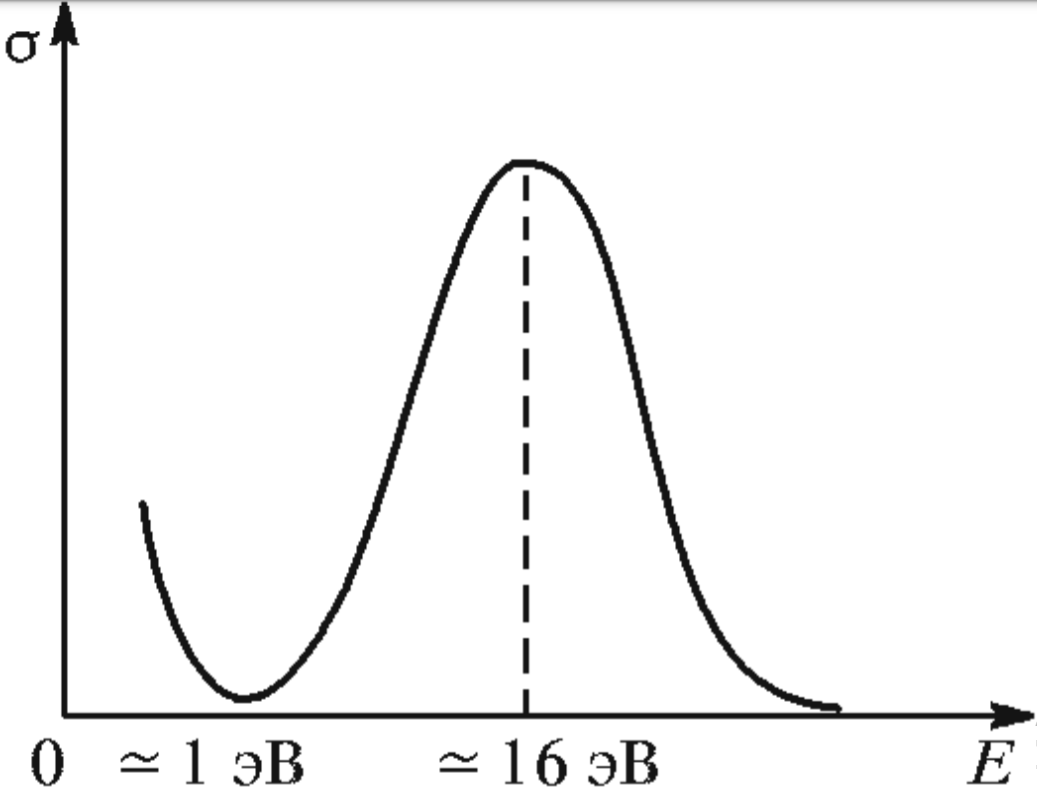
\includegraphics[width=\linewidth]{sigma.png}
  \label{pic::sigma}
  \caption{Качественная картина результатов измерения упругого рассеяния
  электронов в аргоне}
\end{wrapfigure}

Таким образом, сечение имеет размерность площади.
Качественно результат экспериментов Рамзауэра при энергии электронов порядка
десятков электрон-вольт на аргоне показан на рис. (\ref{pic::sigma}). По мере
уменьшения энергии электрона от нескольких десятков электрон-вольт поперечное
сечение его упругого рассеяния растет, как это и следует измеренными очень простых
рассуждений: чем меньше скорость электрона, тем медленнее он <<проскакивает>>
мимо атома, тем больше вероятность этого взаимодействия, т.е. сечение реакции.

Однако в эксперименте наблюдалось, что при энергиях меньше 16 эВ сечение
начинает уменьшаться, а при $E \approx 1$ эВ практически равно нулю, т.е. аргон
становится прозрачным для электронов. При дальнейшем уменьшении энергии
электронов сечение рассеяния опять начинает возрастать.

Последующие опыты показали, что это удивительное поведение поперечного сечения
свойственно не только атомам аргона, но и атомам всех инертных газов. Такое
поведение электронов нельзя объяснить с позиций классической физики.

\begin{wrapfigure}[13]{l}{0.4\linewidth}
  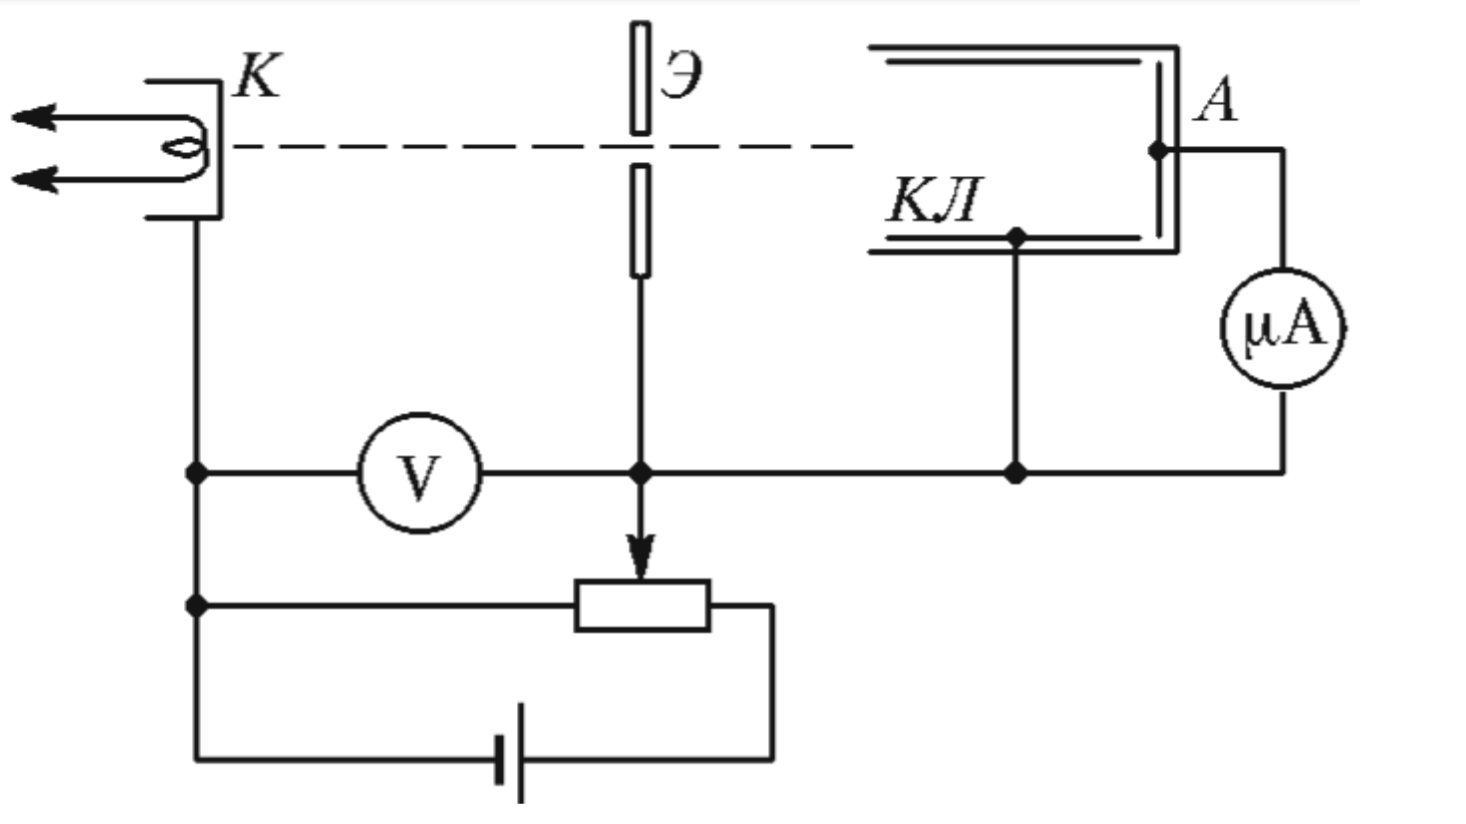
\includegraphics[width=\linewidth]{scheme.png}
  \caption{Схема установки для измерения сечения рассеяния электронов в газах}
  \label{pic::scheme}
\end{wrapfigure}

Схема эксперимента Рамзауэра показана на рис. (\ref{pic::scheme}). Пучок
электронов, вылетая из накаленного катода $K$, проходит ускоряющую разность
потенциалов $V$, приложенную между катодом и электродом, и приобретает тем самым
энергию $E = \frac{m \upsilon^2}{2} = eV$. При прохождении через газ часть
электронов рассеивается на атомах, уходит в сторону и собирается коллектором, а
прошедшие без рассеяния электроны попадают на анод $A$ и создают анодный ток
$I$. Ток $I$ пропорционален числу прошедших электронов, и поэтому
непосредственно характеризует проницаемость газа для электронного пучка в
зависимости от его скорости (ускоряющего напряжения). Согласно классическим
воззрениям с ростом напряжения $V$, как указывалось выше, сечение рассеяния
уменьшается, и ток должен монотонно возрастать.

С точки зрения квантовой теории картина рассеяния выглядит иначе. Внутри атома
потенциальная энергия налетающего электрона $U$ отлична от нуля, скорость
электрона изменяется, становясь равной $\upsilon'$ в соответствии с законом
сохранения энергии

\begin{equation} \label{energy}
  E = \frac{m \upsilon^2}{2} = \frac{m \upsilon'}{2} + U
\end{equation}

а значит, изменяется и длина волны де Бройля. Таким образом, по отношению к
электронной волне атом ведет себя как преломляющая среда с относительным
показателем преломления

\begin{equation}
  n = \frac{\lambda}{\lambda'} = \sqrt{1 + \frac{U}{E}}
\end{equation}

Рассмотрим грубую модель: будем считать, что электрон рассеивается на одномерной
потенциальной яме конечной глубины. Форму реального потенциала для качественных
оценок можно считать прямоугольной. Модель прямоугольной потенциальной ямы
является хорошим приближением для атомов тяжелых инертных газов, отличающихся
наиболее компактной структурой и резкой внешней границей.

Уравнение Шрёдингера в данном случае имеет вид

\begin{equation}
  \psi'' + k^2 \psi = 0, \text{где} \: k^2 =
  \left\lbrace
  \begin{matrix}
    k_1^2 = \frac{2 m E}{h^2} - \text{в областях \RomanNumeralCaps{1} и \RomanNumeralCaps{2}}\\
    k_2^2 = \frac{2 m (E + U_0)}{h^2} - \text{в области \RomanNumeralCaps{3}}
  \end{matrix}
  \right.
\end{equation}

Коэффициент прохождения равен отношению квадратов амплитуд прошедшей и падающей
волн и определяется выражением

\begin{equation}
  D = \frac{16 k_1^2 k_2^2}
  {16 k_1^2 k_2^2 + 4 (k_1^2 - k_2^2)^2 \sin^2(k_2 l)}
\end{equation}

или

\begin{equation}
  D^{-1} = 1 + \frac{(k_1^2 + k_2^2)^2}{4 k_1^2 k_2^2}
   = 1 + \frac{U_0^2}{4 E (E + U_0)} \sin^2 (k_2 l)
\end{equation}

\begin{figure}
  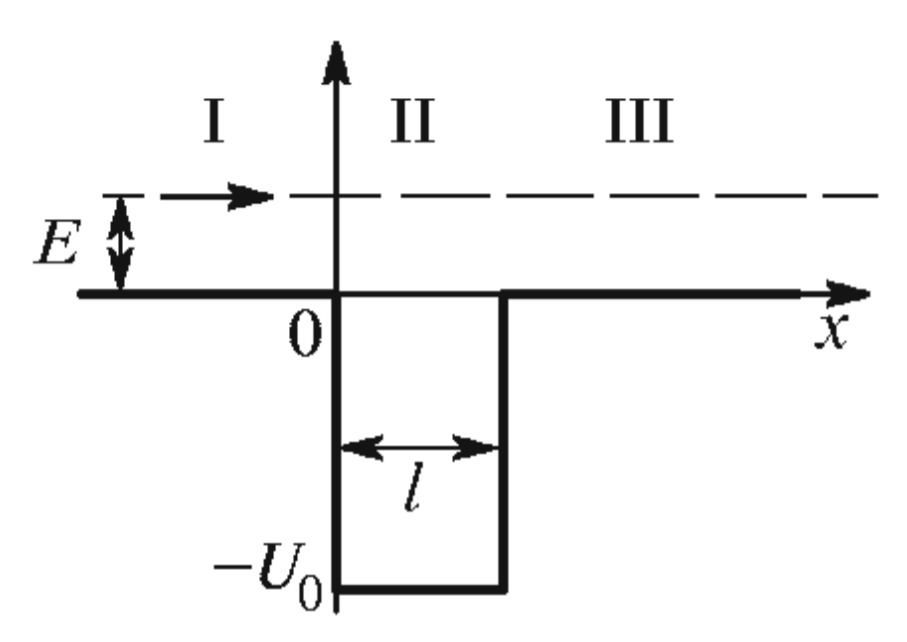
\includegraphics[width=0.5\linewidth]{fall.png}
  \caption{Схематическое изображение прямоугольной ямы, над которой пролетает
  частица с энергией $E$}
  \label{pic::fall}

  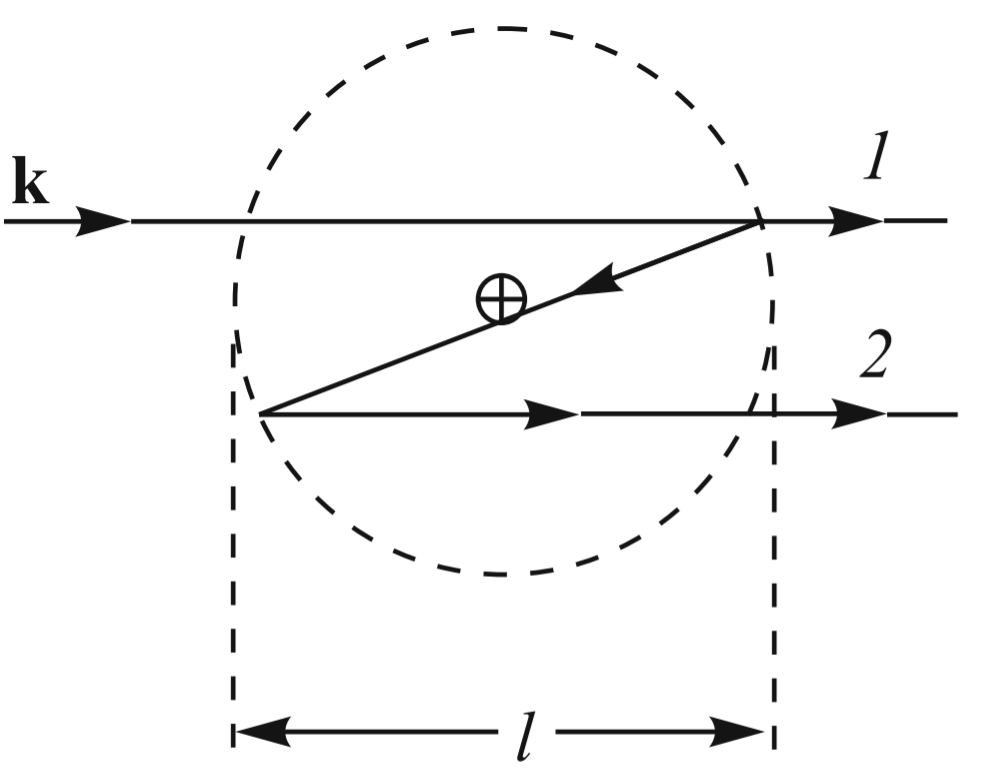
\includegraphics[width=0.5\linewidth]{intefr.png}
  \caption{Схема интерференции волн де Бройля при рассеянии на атоме}
  \label{pic::interf}
\end{figure}

Мы видим, что коэффициент прохождения частицы над ямой имеет, в зависимости от
ее энергии, ряд чередующихся максимумов и минимумов. В частности, если $k_2 l -
\pi$, то $\sin k_2 l = 0$ и коэффициент прохождения равен единице, т.е.
отраженная волна отсутствует, и электрон беспрепятственно проходит через атом,
что является квантовым аналогом просветления оптики.

Таким образом, коэффициент прохождения электронов максимален при условии

\begin{equation} \label{eq::max_cond}
  k_2 l = \sqrt{\frac{2 m (E + U_0)}{\hbar^2}} \cdot l = n \pi, \: n = 1, 2, 3 \dots
\end{equation}

Это условие легко получить, рассматривая интерференцию электронных волн де
Бройля в атоме. Движущемуся электрону соответствует волна де Бройля, длина
которой определяется соотношением $\lambda = h / m \upsilon$. Если кинетическая
энергия электрона невелика, то $E = m \upsilon^2 / 2$ и $\lambda = h / \sqrt{2 m
E}$. При движении электрона через атом длина волны де Бройля становится меньше и
равна $\lambda'= h / \sqrt{2 m (E + U_0)}$, где $U_0$ -- глубина атомного
потенциала. При этом, как показано на рис. (\ref{pic::interf}) волна де Бройля
отражается от границ атомного потенциала, т.е. от поверхности атома, и
происходит интерференция прошедшей через атом волны $1$ и волны $2$, отраженной
от передней и задней границы атом (эти волны когерентны).

Прошедшая волна $1$ усилится волной $2$, если геометрическая разность хода между
ними $\Delta = 2l = \lambda'$, что соответствует условию первого
интерференционного максимума, т.е. при условии

\begin{equation} \label{eq::first_max_cond}
  2l = \frac{h}{\sqrt{2m(E_1 + U_0)}}
\end{equation}

Здесь $E_1$ -- энергия электрона, соответствующая этому условию, которое
совпадает с условием \eqref{eq::max_cond}, следующим из решения уравнения
Шрёдингера.

С другой стороны, прошедшая волна ослабится, если $\Delta = 2l = (3/2)\lambda'$
(условие первого интерференционного минимума), т.е. при условии

\begin{equation} \label{eq::first_min_cond}
  2l = \frac{3}{2} \cdot \frac{h}{\sqrt{2m(E_2 + U_0)}}
\end{equation}

Решая совместно эти два уравнения, можно исключить $U_0$ и найти эффективный
размер атома $l$

\begin{equation}\label{eq::l_3}
  l = \frac{h \sqrt{5}}{\sqrt{32m(E_2 - E_1)}}
\end{equation}

Понятно, что энергии $E_1$ и $E_2$ соответствуют энергиям электронов, прошедших
разность потенциалов $V_1$ и $V_2$, т.е. $E_1 = e V_1$ и $E_2 = e V_2$.

Из формул \eqref{eq::first_max_cond} и \eqref{eq::first_min_cond} можно также по
измеренным величинам $E_1$ и $E_2$ рассчитать эффективную глубину потенциальной
ямы атома:

\begin{equation}\label{eq::Umin}
  U_0 = \frac{4}{5} E_2 - \frac{9}{5} E_1
\end{equation}
